%
% RELATED NOTES (Richard)
%    PersonalJBArchive
%    PSnucleosynthesis/Branch-GalaxyAssemblyAndZDistribution 
%        */bhmetals   : paper.tex, paper-shorter.tex
\documentclass[nofootinbib,twocolumn,prd]{emulateapj}
\usepackage{hyperref}
\usepackage{amsmath}
\usepackage{graphicx}
\usepackage{color}
\usepackage{ifpdf}
%\usepackage{eps2pdf}

\newcommand\mc{{\cal M}_c{}}
\newcommand\editremark[1]{{\color{red}#1}}
\newcommand\msun{M_\odot}
\newcommand\unit[1]{\text{#1}}
\newcommand\abbrvPSgrb{PSG}
\newcommand\abbrvPSellipticals{PSE}
\newcommand\abbrvKBLowZa{BD2010}
\newcommand\ForInternalReference[1]{}
\newcommand\modelDefault{A}
\newcommand\modelNiino{A'}
\newcommand\modelKW{D}
\newcommand\modelMannucci{D'}
\newcommand\modelKB{B}
\newcommand\modelPanter{C}
\newcommand\cqg{CQG}
%\newcommand\aap{A\&A}
%\newcommand\apss{APSS}
%\newcommand\aaps{AAPS}
%% \newcommand\apjs{ApJ S}
%% \newcommand\aj{AJ}
%% \newcommand\apjl{ApJL}
%% \newcommand\mnras{MNRAS}
%% \newcommand\pasp{PASP}
%% \newcommand\pasj{PASJ}
%% \newcommand\araa{ARAA}
%% \newcommand\physrep{Phys. Rep.}


\begin{document}
\title{Details matter: Similar-looking host galaxies can produce different merging compact binary populations} 
\author{R.\ O'Shaughnessy}
\affiliation{Center for Computational Relativity and Gravitation, Rochester Institute of Technology, Rochester, NY 14623, USA}
\email{oshaughn@mail.rit.edu}
\author{ J. Bellovary}
\affiliation{Department of Physics and Astronomy, Vanderbilt University, Nashville TN 37235}
\email{jillian.bellovary@vanderbilt.edu}
\begin{abstract}
% POINT:
% - existence proof by example .. not an attempt to solve the general problem we raise
Galaxy formation
simulations can reproduce present-day galaxies with notably different assembly and star formation histories.  
Recent binary evolution simulations suggest the compact binary merger rate depends
sensitively on the progentior's metallicity, to the extent that rare low-metallicity star formation during galaxy
assembly can produce more detected compact binaries than typical star formation.   
Using detailed simulations of galaxy and chemical evolution, we demonstrate by example that galaxies with similar present-day appearance can host distinctly different
compact binary populations.
We discuss the implications for transient multimessenger astronomy with compact binary sources. 
%% Present and future observations of  merging compact binaries can provide valuable constraints on their birthrate
%%  and formation scenarios.  However, recent binary evolution simulations suggest the compact binary merger rate depends
%% sensitively on the progentior's metallicity, to the extent that rare low-metallicity star formation during galaxy
%% assembly can produce more detected compact binaries than typical star formation.    Additionally, galaxy formation
%% simulations can reproduce present-day galaxies with notably different assembly and star formation histories, with
%% corresponding different present-day merger rates.  
%% % POINT 0: Gasoline + popsyn: real work was done
%% Using existing simulations of the assembly,  chemical evolution, and compact-object formation rate of a single halo
%% Milky Way-like galaxy with Gasoline, we construct present-day compact binary merger rates using a simple semianalytic
%% compact binary formation model ($dP/dt \propto Z^\alpha/t $) motivated by detailed calculations in the literature. 
%% % POINT 1: Observations
%% %   - difficult to reconstruct f
%% %   - local particle far away
%% As expected, we show the present-day galactic state can be only weakly correlated with the dominant compact binary
%% fomation rate: the galaxy could form in several ways, including epochs of low-metallicity star formation through major
%% mergers; and present-day mergers rarely occur near gas with their progenitor metallicity, even when not kicked.  
%% %  - but the galaxy 
%% By contrast,  detailed studies which reconstruct the galaxy's star formation history and metallicity evolution could,
%% when stacked, pinpoint the dominant formation process \editremark{need more than handwaving}.
% POINT 2: Revised merger rates
%% Averaging over the cosmological star formation history and galaxy mass-metallicity relation, we demonstrate low
%% metallicity star formation can produce much of the detected population of short GRBs and nearly all gravitatational-wave
%% sources. 
%% % POINT 3: Challenge for observations
%% Therefore,  though a potentially large fraction of binaries formed from low-metallicity gas,  their birth metallicity
%% cannot be identified directly, even with spatially resolved observations. 
%% %
%% We discuss the extent to which observations can distinguish between different scenarios for  low-metallicity compact
%% binary formation.
%
%\textbf{say something using GRBs in paragraph; perhaps mention relative bias in $p(M_g|GRB)$ relative to prior?}
%% \textbf{say something about different SFR histories making present galaxies -- can do more if we can distinguish history
%% of the galaxy}

\end{abstract}

\maketitle

\section{Introduction}
% POINT: LIGO soon will detect compact binary mergers....
%     ... and possibly EM counter part too
%     ... which will enable new physics
In the next few years, ground-based gravitational wave detectors like LIGO 
and Virgo  should detect the gravitational
wave signal from merging compact binaries, including  binary  neutron stars and black hole-neutron star binaries; see,
e.g., \cite{LIGO-Inspiral-Rates} and references therein.
In addition to the strong gravitational wave signal, mergers of neutron stars are expected to  frequently be accompanied by detectable
electromagnetic radiation  via a number of  mechanisms, including a strong but tightly beamed
ultrarelativistic jet and weakly-beamed but more isotropic thermal radiation from an expanding hot shell
\citep[see,e.g.,][and references therein]{2013PhRvL.111r1101C,short-grb-GWCoincidenceEM-MetzgerBerger2011}.  
% People we can't afford the space to cite, alas:
%    - 2015arXiv150101986H   -
%    - 2013MNRAS.430.2121P - Rosswog recent
%    - Shibata group/Koutarou
In addition to providing a wealth of information about the merger event itself, a multimessenger detection will pin down
the sky position and therefore approximate birthplace of each merging binary.    
As with supernovae and  GRBs, these host galaxy associations   are expected to tightly constrain models for compact binary
formation; see, for comparison,  \citet{2011MNRAS.412.1508M}, \citet{long-grb-GuettaPiran2007},
\citet{2014ARAA..52...43B}, and references therein. %2010ApJ...722.1879M,2010MNRAS.407.1314M}.     
%

% POINT: Huge detail possible
The host galaxies of distant short GRBs have already been extensively investigated, with the associations being used to
draw preliminary conclusions about their progentitors  \cite{2014ARAA..52...43B}.   
%Of necessity, these analyses  on bulk correlations, often stacked to increase significance across multiple sources
%\editremark{clean up/don't piss off   Edo}.  
Unlike GRBs, detected gravitational wave sources will be limited by the range of LIGO to the local universe; for
example,  binary neutron star sources should be closer than $400\unit{Mpc}$.  Due to their proximity, each host galaxy
can be explored at great depth and detail via  position-resolved spectroscopy, enabling detailed position-resolved star-formation
and chemical evolution histories \editremark{citation: need better ones} \citep[see,e.g.][]{2009MNRAS.396..462K,2014MNRAS.444..336C}.
% POINT: But is it useful?
In this work, we demonstrate by concrete example that detailed analysis of individual galaxies can be essential to
investigate key physical questions about the origin of compact binary mergers. 


This paper is organized as follows. 
In \S \ref{sec:sims}, we describe detailed hydrodynamical simulations of  two galaxies.  Though these two
galaxies are at  present similar to the Milky Way, we
show that their star formation and chemical evolution history have subtle but important differences due to their
distinctive merger histories.   To demonstrate
these differences have a significant practical impact,  in \S \ref{sec:model}, we introduce a simple,
metallicity-dependent  phenomenological model to calculate the present-day rate and mass distribution of compact binary
mergers from  a galaxy's known history.  
In \S \ref{sec:results} we show that while these two galaxy formation models should produce comparable detectable binary neutron star
populations, these two scenarios could produce dramatically different populations of electromagnetically detectable
merging black hole-neutron star binaries. 
%


%% %   - Delay  time only: 
%% For example, the lag between transients' redshift distribution and the past star formation rate has shown long GRBs are
%% associated with short-lived progenitors (see, e.g., \cite{long-grb-GuettaPiran2007} \cite{grb-long-Virgili2011-TryingEverything} and
%% references therein) and that SNIa merge long after their formation
%% \citep{sn1a-DelayTimeDistribution-Cosmological-Graur2011}. \editremark{other cites}
%% % * \cite{YoungLongGRBHostPredictions2007,FryerGRBProgenitorConstraints2007} : Long bursts.
%% By contrast, short GRBs noticably lag cosmological star formation  \editremark{Berger; }\cite{2007ApJ...665.1220Z,Nakar} 




\section{Cosmological simulations produce two distinct Milky-Way-like galaxies}
\label{sec:sims}

\subsection{Simulating galaxy evolution}
To thoroughly examine the significance of low metallicity star
formation, we have run a cosmological smoothed particle hydrodynamics
(SPH) $N$-body simulation of a Milky Way-like galaxy with GASOLINE
\citep{Stadel01,Wadsley04}.  This simulation allows us to analyze both
spatially and temporally resolved star formation, and determine not
only the metallicity history of compact object progenitors, but also
their dynamical evolution.  One simulation we report here, $h258$,
involves the formation of a Milky Way-like disk galaxy whose
progenitors undergo major mergers at $z = 2$ and $z = 0.8$.  This
simulation has been previously discussed by
\citet{Governato09,Bellovary10,Bellovary11,Brooks11}; however we have
re-run the simulation at a factor of two higher in spatial resolution
and additionally included new physics including a prescription for
cooling by molecular hydrogen (Christensen et al. in prep).

We selected our simulated region of interest from a 50 Mpc volume of
uniform resolution, and resampled the region of interest at very high
resolution using the volume renormalization technique \citep{Katz93}.
This technique allows us to follow the detailed physical processes
involved in galaxy evolution in our selected region while still
including large-scale torques from cosmic structure.  We use {\bf
WMAPX} cosmology \citep{WMAP} and model the ionizing UV background
with the prescription from \citet{Haardt96}.  Stars form
probabilistically from gas particles which meet density ($n_{min} =
10$ amu cm$^{-3}$) and temperature ($T_{max} = 10^4$ K) thresholds
{\bf (additional description needed for H2 SF prescription)}. If a gas
particle meets these criteria, it has a likelihood of forming a star
particle (representing a simple stellar population with a Kroupa IMF
\citep{Kroupa}) which is given by

\begin{equation}
p = \frac{m_{\rm gas}}{m_{\rm star}} (1 - e^{c^*\Delta t/t_{\rm form}})
\end{equation}

\noindent
where the star formation efficiency parameter $c^*$ is set to 0.1 such
that our galaxies match the observed Kennicutt-Schmidt law
\citep{Kennicutt89}; $m_{star}$ and $m_{gas}$ are the star and gas
particle masses;\footnote{In our high-resolution simulations \textbf{ROS-check!}, each gas particle starts with a mass
  $m_{gas,0}=26,676 M_\odot$, gaining mass from feedback and losing it to star formation.  Each star particle, when
  formed, has $1/3$ of the progenitor mass of the forming gas particle.  See \cite{2010ApJ...717..121C} for a discussion
of resolution issues in these SPH simulations.} $t_{form}$ is the dynamical time for the gas
particle; and $\Delta t$ is the time between star formation episodes,
which we set to 1 Myr.  We model supernova feedback using the
blastwave formalism described in \citet{McKee77} and implemented in
our simulations as in \citet{Stinson06}.  Each supernova releases
$E_{SN} = 10^{51}$ erg into the surrounding gas with a radius
determined by the blastwave equations.  These particles are not
allowed to cool for the duration of the blastwave, mimicking the
snowplow phase of a supernova explosion.  Previous works have found
that this set of parameters results in realistic galaxies which obey a
number of observed relations such as the mass-metallicity relation
\citep{Brooks07}, the Tully-Fisher relation \citep{Governato09}, and
the size-luminosity relation \citep{Brooks11}, as well as reproduce
the detailed characteristics of bulgeless dwarf galaxies
\citep{Governato10} and the Milky Way \citep{Guedes11}.


Also included in our simulations is a scheme for turbulent metal
diffusion \citep{Shen10}.  Metals are created in supernova explosions
and deposited directly to the gas within the blast radius.  Stellar
masses are converted to ages as described by \citet{Raiteri96}, and
stars more massive than 8 M$_\odot$ are able to undergo a Type II
supernova.  We follow metal enrichment from both Type II and Type 1a
supernova, with metal yields derived from \citet{Weaver93} and
\citet{Thielemann86} respectively.  From this point onwards metals
diffuse through the surrounding gas, according to 
\begin{equation}
\frac{dZ}{dt}|_{diff} = \nabla (D \nabla {Z}) \\
\end{equation}
%
where the diffusion paremeter $D$ is given by
%
\begin{equation}
D = C_{diff} |S_{ij}| h
\end{equation}
%
and $h$ is the SPH smoothing length, $S_{ij}$ is the trace-free shear
tensor, and $C_{diff}$ is a dimensionless constant which we set to
{\bf something.  Reasons for setting it are good, let's have some.
Sijing finds that C = 0.05 makes for a good comparison to clusters, we
tend to use something more conservative}.

We identify individual galaxies using the halo finder $AHF$
\citep{Gill04,Knollmann09}, which identifies halos based on an
overdensity criterion for a flat universe \citep{Gross97}.  For this
work, we are focusing on the primary (i.e. most massive) galaxy at any
given redshift, which serves as the progenitor to our $z = 0$ Milky
Way-like galaxy.



\subsection{Two Milky-Way-like galaxies with distinct histories }

{\bf Richard go ahead and edit this however is needed.}  The evolution
of a galaxy, in terms of its stellar mass and metallicity evolution,
depends strongly on its interaction history.  Galaxies which look
similar at the present day may have had drastically different
histories, which may result in differences in compact object merger
rates.  To investigate whether galaxy history affects the GRB event
rate, we have chosen two simulations which are extremely similar at $z
= 0$ but differ strongly in their merger histories.

The simulation h277 (Boring Galaxy) is a Milky Way analog with a
quiescent merger history.  It experiences its last major merger at $z
= 3$, after which a small number of minor interactions permeate its
life.  This simulation has been shown to emulate several Milky Way
properties, including stellar dynamics
\citep{Loebman12,Loebman14,Kassin14}, baryon fraction
\citep{Munshi13}, halo properties \citep{Zolotov09,Zolotov10}, and
  disk properties \citep{Brooks11}.  It has a virial mass of $M_{vir}
  = 6.79 \times 10^{11}  \msun$, stellar mass $M_* = 4.24 \times
  10^{10} \msun$, and circular velocity $v_{circ} = \editremark{xx}$ km s$^{-1}$.

  The simulation h258 (Exciting Galaxy), on the other hand, has a much
  more active merger history.  At $z = 1$ there is a 1:1 merger event;
  a gas disk rapidly reforms following the collision (see
  \citet{Governato09}), resulting in a massive disk galaxy at $z = 0$
  which looks remarkably similar to the Milky Way and to the other
  simulation, h277.  Prior to the $z = 1$ merger, each of the two
  progenitor galaxies actually experiences its own additional major
  merger events around $z = 2.5$ ({\bf check!}).  The combination of
  the series of major mergers, plus a number of minor interactions and
  flybys, gives a stark contrast to the relatively quiescent history
  of h277.  At $z = 0$, h258 has a virial mass of $M_{vir} = 7.74
  \times 10^{11} \msun$, stellar mass $M_* = 4.46 \times 10^{10}$
  \msun, and circular velocity $v_{circ} = \editremark{xx}$ km s$^{-1}$.


  Due to the differences in merger histories, the metallicity
  evolution of h258 and h277 also differ at early times.  Figure
  \ref{fig:TwoGalaxies} shows the history of the mean metallicty of
  recently formed stars vs time (thick solid lines), where we define
  recent as within the past 50 Myr.  The shaded regions correspond to
  one standard devation of the mean, while the thick dashed lines
  represent the top and bottom 90\%.  We see that {\bf different things happen at different times.}



\begin{figure*}
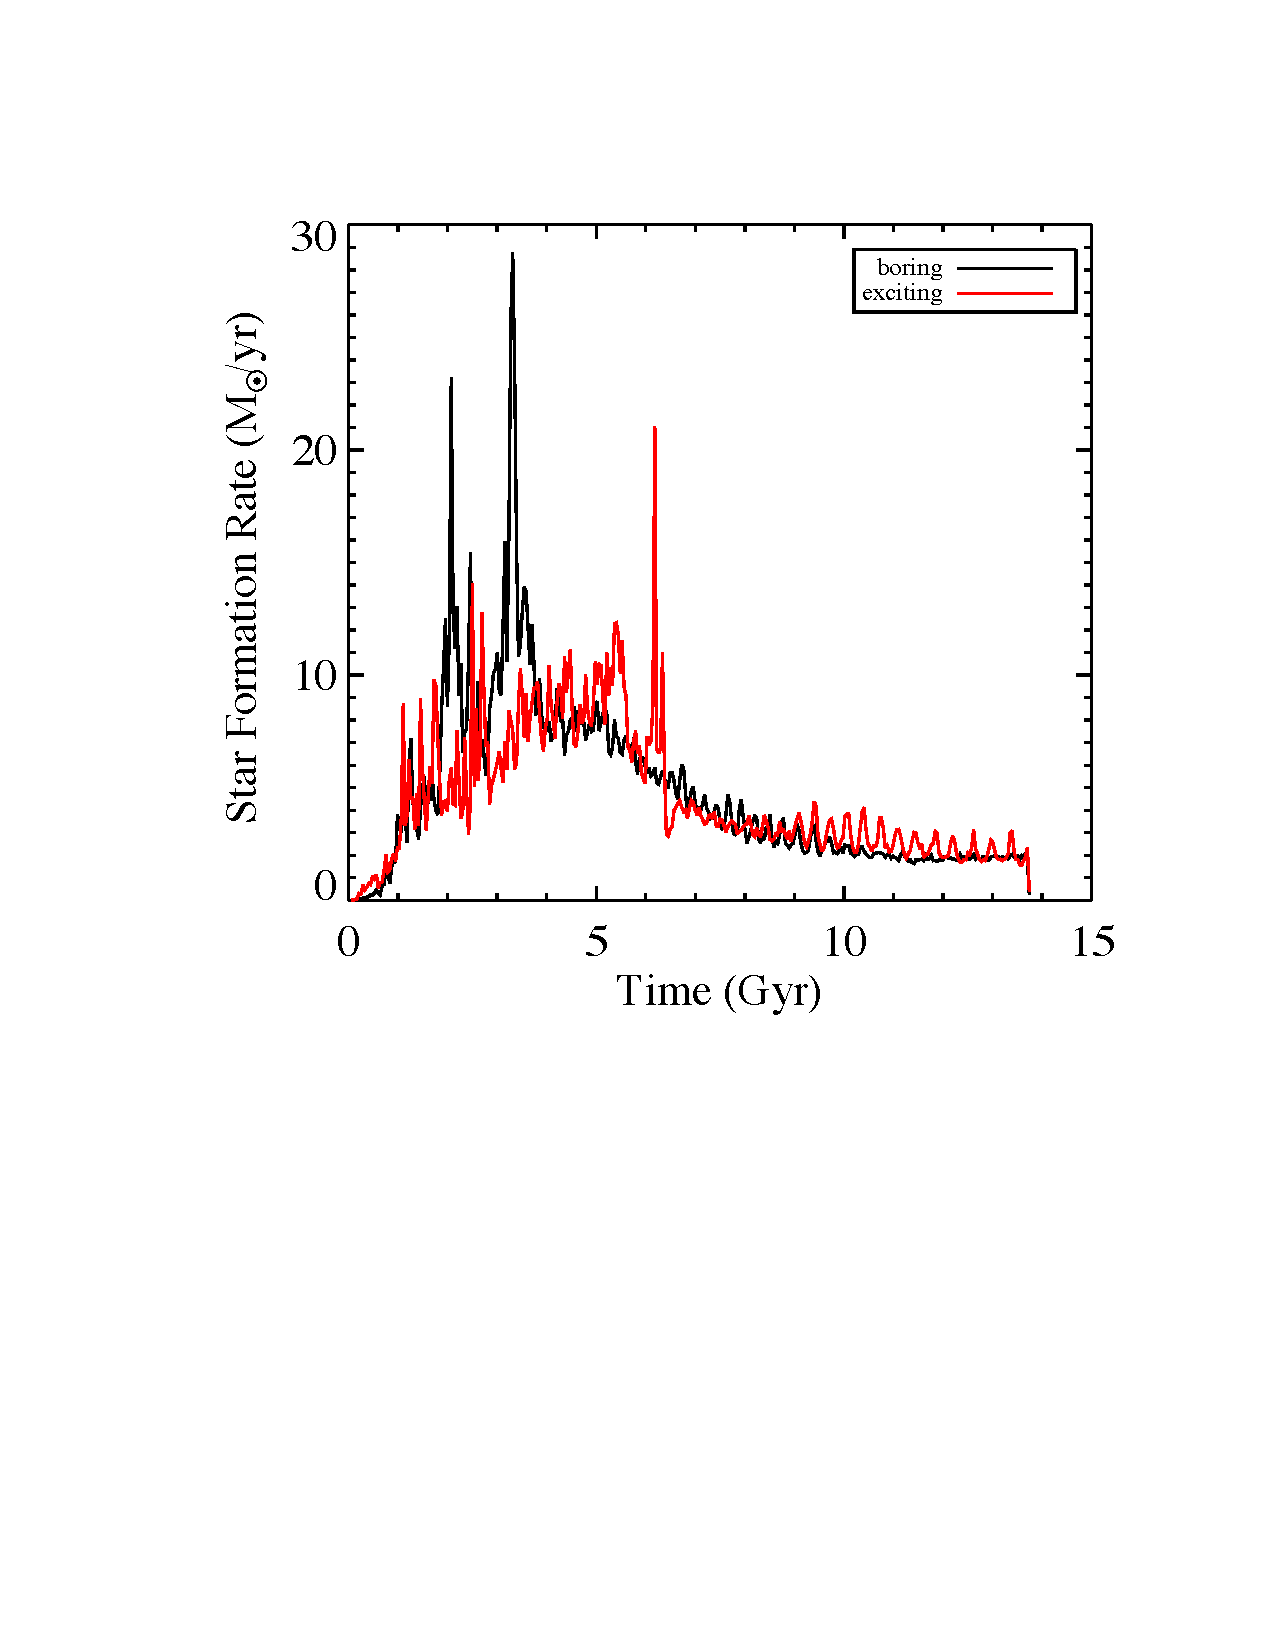
\includegraphics[width=\columnwidth]{Figures/sfh}
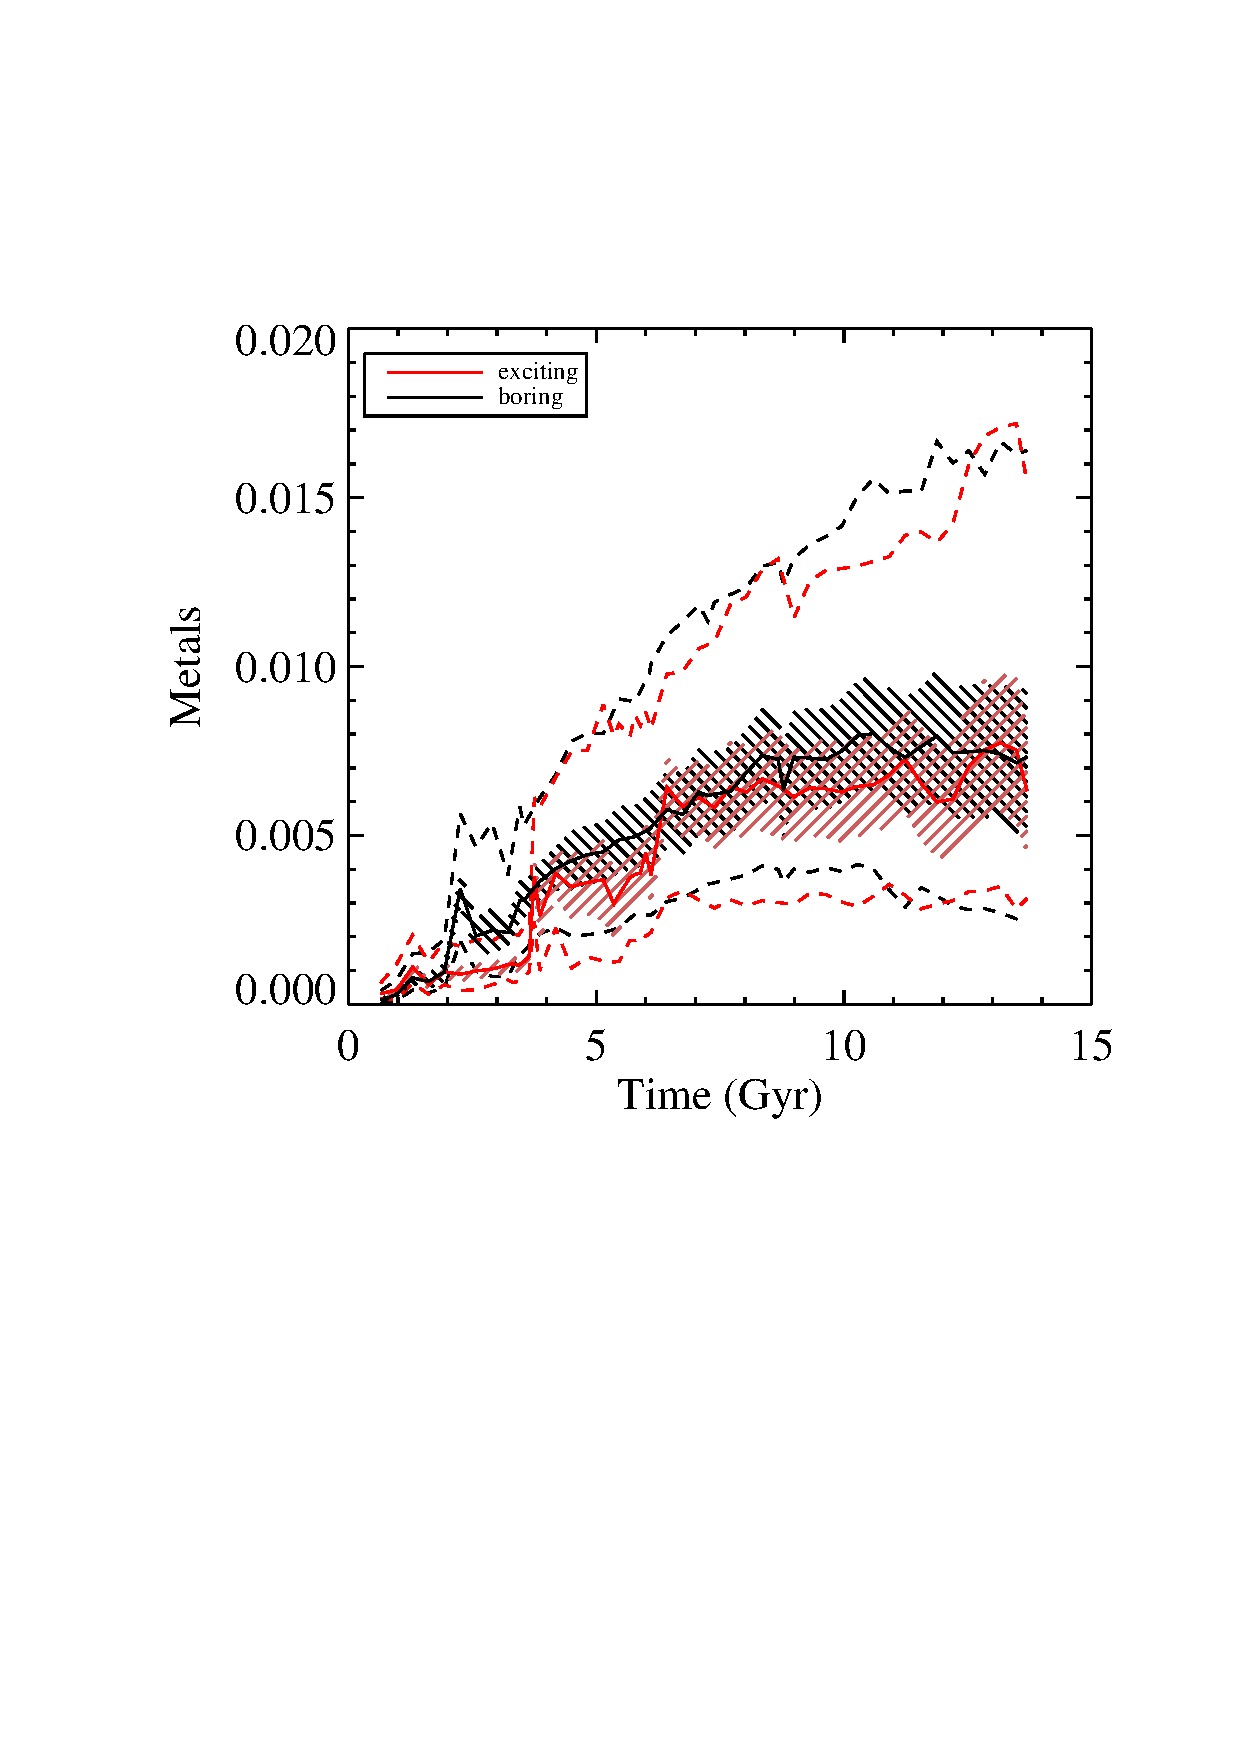
\includegraphics[width=\columnwidth]{Figures/zvst}
\caption{\label{fig:TwoGalaxies}\textbf{Star formation and metallicity versus time}:  \emph{Left panel}: Star formation history $\dot{M}_{*}$
  versus time.  Black corresponds to galaxy A (``boring'') and red to gaalxy B (``exciting'').  
\emph{Right panel}: A plot of the  metallicity $Z$ of recently-formed stars versus time.  Solid red and black lines show
the mean metallicity; dotted lines correspond to  90\% of newly-born stars have lower metallicity,   or 10\% of
newly-born stars have greater metallicity.  When these two galaxies are $2-3\unit{Gyr}$ old, prior to the first major
merger of  near the peak of their
star-forming history, newly-born stars are created with significantlydifferent metallicity.  Additionally, prior to the
second major merger of galaxy B at $\simeq 6\unit{Gyr}$, stars form in the ``exciting'' galaxy at a systematically lower
metallicity than in the ``boring'' counterpart.
}
\end{figure*}

\section{Model for compact binary formation}
\label{sec:model}


Binary evolution calculations suggest the detection rate depends sensitively on the assumed metallicity, in conjuction
with other parameters \citep[see,\,e.g.][and references
  therein]{popsyn-LowMetallicityImpact-Chris2008,popsyn-LIGO-SFR-2008}.\editremark{New dominik et al}
% POINT: 
%   - final BH spin, mass can change number favored
%   - of course
The detected population of compact binary mergers can further favor low-metallicity environments, e.g. through the total
mass of merging binaries.
% POINT: Simple model to encompass all
To explore plausible binary detection scenarios, we adopt a parameterized formalism for binary evolution and event detection, motivated by
the detailed studies of  \abbrvPSgrb{} and \abbrvPSellipticals.  Specifically, we encapsulate all information about
 binary evolution into two  parameterized response functions.  The funciton ${\cal G}(t| Z) =
dN/dt dM_*$ describes how many mergers per unit initial mass occur after a time $t$ since a starburst,
given ambient metallicity $Z$.  The function $p(m_1,m_2|Z)$ is a metallicity-dependent mass distribution for binaries
formed in a metallicity $Z$.
%
Finally, we account for the substantially increased sensitivity of gravitational wave detectors to binaries of larger
chirp mass $\mc=(m_1 m_2)^{3/5}/(m_1+m_2)^{1/5}$; see \abbrvPSellipticals.
%
In terms of this response function, we can therefore calculate the relative contribution to the LIGO  event rate $r_D$
due to any individual galaxy via the following formula 
\begin{widetext}
\begin{subequations}
\label{eq:RatePerGalaxy}
\begin{eqnarray}
r_D  &\equiv& \int^{0}_{-T_{univ}} dt' d\log Z  \, [\dot{M}_*(t') p(\log Z|t) ] \times \; {\cal G}(0-t' | Z)  
 [\int d\mc p(\mc|Z) (\mc/1.2 M_\odot)^{15/6}]
%\\
%% {\cal R}(z)&\equiv &  \int dx {\cal R} p(z)
\end{eqnarray}
\end{subequations}
\end{widetext}
In this expression, the galactic star formation rate
$\dot{M}_*$ and star formation metallicity distribution $p(\log Z|t)$ are galaxy-dependent and drawn from our
simulations.   \editremark{rewrite this to be average chirp mass at a given metallicity}


We parameterize the response function ${\cal G}(t|Z)$ with two factors: (a) an overall efficiency $\lambda$ for forming
binaries;  and (b) a
cumulative delay time distribution $P_t(<t|Z)$, describing the fraction of binaries born at $t=0$ that merge in less
than time $t$ from a population of binaries $Z$:\footnote{For simplicity, we assume the mass and delay time
  distributions are uncorrelated.  Figure A9 in \abbrvPSgrb{} shows this approximation, while not strictly true, is an
  excellent approximation for merging BH-BH binaries at solar metallicity.  }
\begin{eqnarray}
G(t,x|Z) &=& \lambda(Z) p_x(x|Z) \frac{dP_t}{dt}(t) 
\end{eqnarray}
Previous studies suggest the number of merging compact binaries $\lambda \delta M_*$ produced by a starburst depends
as a power law on metallicity:
\begin{eqnarray}
\label{eq:LambdaVersusZModel}
\lambda(Z) &=& \lambda_o \text{max}[(Z/Z_\odot)^{-a}, F_{max}] 
\end{eqnarray}
with $a\in [0,3]$ and $F_{max}<10^3$
%$\lambda_o F_{max} < 3\times 10^{-4}/M_\odot$
 (see, e.g.\cite{popsyn-LIGO-SFR-2008}, \abbrvKBLowZa).
In this paper we only investigate the dependence of rates with metallicity; we therefore  adopt 
\[
\lambda_0 = 10^{-3}/M_\odot
\]
as a typical value for neutron star compact binaries (see \abbrvPSgrb{}, \abbrvPSellipticals, and \abbrvKBLowZa).
%
Finally, for simplicity we adopt the universal delay time distribution
%% Finally, we parameterize the delay time distribution by  either
%% \begin{eqnarray}
%% P_t(<t) &=& \begin{cases}
%% 0 & t<10 \unit{Myr} \\
%% (t/13\unit{Gyr})^{b}& t \in [10\unit{Myr},t_H]
%% \end{cases} 
%% \end{eqnarray}
%% with $b> 0$ or as the special case
\begin{eqnarray}
\frac{dP_t(<t)}{dt} =  \begin{cases}
0 & t<10 \unit{Myr} \\
\frac{1}{t \ln (13 \unit{Gyr}/10\unit{Myr})} & t \in [10\unit{Myr},13\unit{Gyr}]
\end{cases} 
\end{eqnarray}
\abbrvPSgrb{} and \abbrvPSellipticals{} show this distribution is reasonable approximations to compact binary delay
time distributions.\footnote{Simulations suggest the delay time distribution varies from model to model and with mass.
  These variations have less impact on our results than the evolving metallicity distribution of star forming gas.}
%
For suitable choices of parameter, our phenomenological response function is qualitatively consistent with the results of detailed simulations of binary
evolution  \citep{2010ApJ...715L.138B,popsyn-LowMetallicityImpact2c-StarTrackRevised-2014,popsyn-LowMetallicityImpact2b-StarTrackRevised-2013,popsyn-LowMetallicityImpact2-StarTrackRevised-2012}.

\subsection{Tidal disruption and black hole mass versus metallicity}
At merger, black holes may promptly engulf a companion neutron star \editremark{same papers as for Brandon:Foucart,
  etc}, unless they have sufficiently small mass and sufficiently large spin.  Without  a tidal disruption event prior to merger, the prospects for associated electromagnetic counterparts
are severely diminished.  
%
A neutron star  (NS) coalescing with a black hole (BH) will be tidally disrupted prior to merger if and only if the component
masses, spins, and equation of state permit it.  As described below, only a small fraction of all  possible coalescing
BH-NS binaries have parameters consistent with tidal disruption.  
%
Stellar evolution and hence supernovae remnants are expected to evolve
substantially with birth metallicity, the black hole mass and possibly spin in black hole-neutron star binaries can depend sensitively on binary formation
channels and the fraction of coalescing NS-BH binaries which are tidally disrupted will vary
over cosmic time. 
%
To quantify this effect, we adopt a simple formula for tidal disruption of neutron stars in BH-NS binaries and a simple
phenomenological model for the metallicity-dependent mass distribution of BHs in BH-NS binaries


\begin{figure}
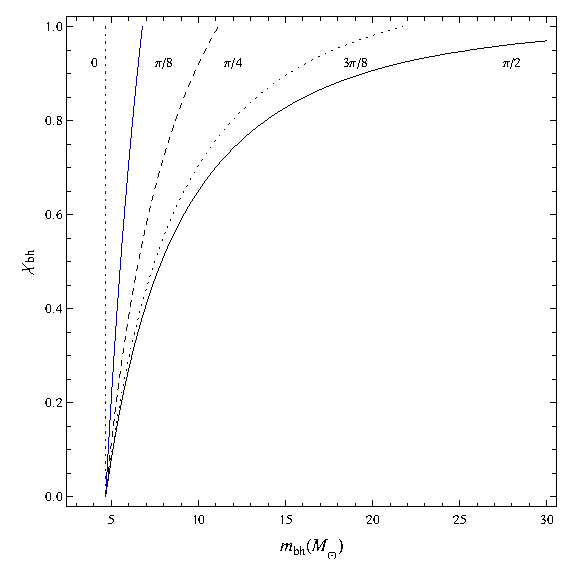
\includegraphics{Figures/fig-mma-TidalDisrupt-MbhA-VersusTheta}
\caption{\label{fig:TidalDisrupt}\textbf{Tidal disruption}:  Following  \citet{2012PhRvD..86l4007F}, a plot of
  the critical spin needed for tidal disruption versus black hole mass and inclination (solid black, dotted black,
  dashed black, solid blue, and dotted blue are $\theta_{LS}=\pi/2,3\pi/8,\pi/4, \pi/8,0$ respectively).  Specifically,
  this figure corresponds to $M_{\rm disk}=0$ in Eq. (\ref{eq:Mdisk}), assuming  a $1.4 M_\odot$ neutron star with compactness ${\cal
    C}=1.66$ in inclined orbit around a spinning black hole of mass $m_{bh}$ and dimensionless spin $\chi_{bh}$.
  Parameters consistent with tidal disruption are above the curves; prompt capture occurs below the
  curve.
}
\end{figure}

% POINT: Trend versus mass and opening angle.  [Be careful: disruption time will depend on opening angle]
To estimate whether a specific compact binary will be tidally disrupted prior to merger, we employ the
following procecure to identify posterior samples consistent with tidal disruption of a neutron star.  First, the
smaller mass must lie within the range of masses allowed by our fiducial NS equation of state (\textbf{MPA1 from Ben}), here
between $0.5 M_\odot$ and $2.5 M_\odot$.  Second, the disruption process must leave behind a remnant disk with nonzero
mass, as estimated using Foucart's expression \cite{2012PhRvD..86l4007F} (his Eqs. (6,12-13)):
\begin{align}
\frac{M_{disk}}{M_{NS}} &=
 0.288 (3 m_{bh}/m_{ns})^{1/3}[1-2 {\cal C}] 
\nonumber \\
&
 -0.148 (m_{bh}/m_{ns})  {\cal C} R_{isco}(a)/m_{bh} 
\label{eq:Mdisk}
\end{align}
where $q=m_{bh}/m_{NS}$ is the binary mass ratio; $a=S_{bh}/m_{bh}^2$ is a dimensionless measure of the black hole spin;
and  where ${\cal C}(m_{ns})=m_{ns}/R_{ns}$ is a mass- and equation-of-state dependent  measure of the neutron star
compactness.  In Foucart's expression, shown above, $R_{isco}(a)$ is the radius of the  innermost stable equitorial circular orbit  of a test particle
about a Kerr black hole  \cite{1972ApJ...178..347B}. % Brandon:  [their Eq. 2.21].   
When the black hole spin is not aligned with the orbit, we use the aligned component of the black hole spin magnitude $a\rightarrow a \cos \theta_{LS}$ in this
expression.   Fixing the neutron star mass $m_{ns}=1.4 M_\odot$ and hence compactness to ${\cal C}=1.66$, this expression implies a two-dimensional surface in
the three-dimensional parameter space $m_{bh},a,\theta_{LS}$ seperates parameters corresponding to tidal disruption to
parameters corresponding to prompt coalescence.
%
After coalescence, the remnant disk generates a tightly beamed electromagnetic counterpart.  For simplicity, we assume
beaming angle is independent of the disruption process or progenitor parameters, so a constant beaming correction factor $f_b$ enters into all
subsequent calculations and can hence be omitted.  
%
Figure \ref{fig:TidalDisrupt} shows contours of this expression for different values of $\theta_{LS}$.

\begin{figure}
\caption{\textbf{Disruption fraction}: Approximate tidal disrpution fraction}
\end{figure}

% POINT: Distribution of tilt angles
Based on Monte Carlo simulations of supernova kicks \editremark{citations:Eggleton,Kalogera,IhmXXX}, we approximate the tilt angle distribution $p(\theta)$ of bound,
coalescing BH-NS binaries by the positive half of a normal distribution
\[
p(\theta)\simeq e^{-\theta^2/2\sigma_\theta^2} \frac{2}{\sqrt{2\pi \sigma_\theta^2}}
\]
where $\sigma_{\theta}\simeq 1$ is a characteristic angular width that varies relatively weakly with the black hole mass
and supernova kick velocity, for velocities consistent with pulsar recoil velocities \editremark{citations}.  This simple distribution is consistent with some detailed population synthesis simulations by
\texttt{StarTrack}. \editremark{validate with more modern startrack}  
For simplicity, in this work we adopt $\sigma_{\theta}=1$.   
%  POINT Average over spin distributions
Using this approximate distribution of misalignment angles, Figure  assumed black hole mass and spin we calculate the
fraction of coalescing binaries consistent with 


% POINT: Average over distributions

The relative probability of a given tilt angle

- first aproximations: tilt angle independent of merger time


% POINT: Include delay time: get examples of disruption fraction versus time




------

\editremark{calibrate mass distribution to synthetic universe/Dominik - but also allow reversed trend}
DISCUSSION: could we explain the redshift distribution of short GRBs this way?


\section{Results}
\label{sec:results}


\begin{verbatim}
ACTION ITEMS AND STATUS

* Result script looks good (\texttt{sfr\_to\_rate.py}).  Follow instructions

** Modify script to include tidal disruption options for BHs

** plot 'stanard' results for NS-NS

** set scale to be physical units -- some ad-hoc factors used

*

* Do we get to different answers?  Are they different ENOUGH?  

** Overall event rate: different by 20\% between two types. Largely similar.
   - plot versus z_exponent.  Is there a trend

** mass-cut-dependent event rate -- will be more sensitive (e.g., if there
  is a hard cutoff on some masses, as having no EM counterpart)
\end{verbatim}


\section{Conclusions}




% POINT: Future directions

\begin{acknowledgements}
ROS acknowledges support from NSF award AST-1412449, via subcontract from the University of Wisconsin-Milwaukee.
%
JB acknolwedges support  from \editremark{writeme}
\end{acknowledgements}

\appendix
\section{Tidal disruption probability}

\section{Outline }
\begin{verbatim}

Intro
  -Important (edo/Brian)
  - More important soon (LIGO; IFU's give detail)
    because these galaxies are local and spatially resolved
    at 400 Mpc distance
  - The question: can we learn about things from detailed host galaxy 
    observations, and if so what?
    Obviously yes (cf. SN Ia, short GRB, etc)
  - Specific questions of interest, particularly for BH-NS origin for short GRBs:
    is there dependence of the event rate and BH mass on the source metallicity

  - Not clear because of kicks, mixing
  - Goal of paper: address this challenge via simulations

Methods
  - JB: specifically target two 'identical' MW galaxies (and their subhalo population)
  - Postproces JB: rhodot; Z of star forming gas
  - Model:
      - predict present-day number (and mass distribution) by formula 

Results:
  - Different histories which look the same now can produce different answers
     - key issue: impact of past mergers
  - 

Stuff to skip
  - (spin-dependent) tidal disruption threshold: assume all BH-NS disrupt, for simplicity
\end{verbatim}
%1 Kilo Parsec/(400 Mega Parsec)
%Convert[%, Milli ArcSecond] // N


\section{Other discussion}


\section{Implications for transient multimessenger astronomy}


% POINT: Observations provide sample of extragalactic  binaries at merger, and  host galaxies.  Possible to mine large archive of events
% to deduce correlations

On the one hand,  relatively few formation scenarios will correctly reproduce the observed mass and spin distributions
\citep{2004MNRAS.352.1372B,2003ApJ...589L..37B,gwastro-Ilya-ConfProc-NRDA-2010}.  
% POINT: Value of associations
%% Green's function connecting the merger
%% rate $dN/dt$ to the star formation rate host galaxy star formation history and metallicity,
%% both the delay time distribution and correlation any preference for different metallicities can be determined
On the other hand, each host galaxy associates a merger to a unique star formation history and metallicity distribution.
With many events, these associations can potentially determine the ``response function'' for compact binaries: how often star forming gas of a given metallicity evolves into
merging compact binaries;  see, e.g., studies of

%
Highly atypical formation scenarios seemingly should produce events in or near atypical hosts.  
% POINT: Introduce *idea* of comparison: refs for mass-metallicity relation
For example, in the local universe galaxies lie along mass-metallicity  (\cite{2004ApJ...613..898T}; see also
\cite{sfr-ZEvolution-ByGalaxy-Panter2008})
or mass-metallicity-star formation rate  correlations (e.g., \cite{2010MNRAS.408.2115M}).
% POINT: Evolution tricky
[The change in these correlations with redshift is still being investigated; see, e.g., \editremark{citation: Panter;
    Mannucci; }, \cite{2011ApJ...739....1L} and references therein.]
% POINT: previous studies
Based on these correlations, both short  and long GRBs seem to arise from
relatively typical hosts at their redshift; see, e.g., \cite{grb-short-Hosts-Berger2008} and \cite{grb-long-HostMetallicityVsTrend-Mannucci2010}.


%  - Host associations: lots of information
Host galaxy associations provide rich information about a transient's present and past environment.
%
For example, in several cases the metallicity of gas neighboring a long GRB (\citet{ 2008AJ....135.1136M}; \citet{2010AJ....140.1557L}
\editremark{links}), short GRB (\editremark{XXX}), or SN has been directly measured.
%
The precise host offset can be compared to the distribution of light and star formation  \citep{2010ApJ...708....9F}.
%
Finally,  on a host-by-host basis, the delay time between birth and merger has been constrained for long GRBs (\editremark{XXX}), short GRBs \citep{2010ApJ...725.1202L}, and
  SN Ia \citep{2011MNRAS.412.1508M}.
%



Biases towards low-metallicity star formation have been extensively studied in the context of long GRBs and their host galaxies.
%
For example, \cite{2009ApJ...702..377K} demonstrated that a sufficiently strong bias towards low-metallicity star formation would predict
most  events in the local universe occur low-mass and dwarf galaxies.
%<
For less extreme metallicity biases, subsequent calculations by  \citet{2011MNRAS.417..567N} demonstrated that the
metallicity distribution within galaxies will usually lead to events in a wide range of host galaxies in the local universe.

\subsection{Local metallicity measurements?}
To this point, we have emphasized \emph{global} measurements of the galactic star formation history.  With the advent of
IFUs and position-resolved spectroscopy, observers can now probe the star formation history and metallicity of
individual gas packets at different points in a galaxy.  
%
These highly-detailed probes will be essential tools to develop a comprehensive model of the galaxy's merger and
chemical evolution history.  That said, the metallicity of stars and gas adjacent to a specific merger event provides
few direct, unambiguous clues to a compact binary merger's progenitors.  
On the one hand, compact binaries are kicked by supernovae, moving substantially away from their birth position
%  2014arXiv1407.3796S : implications for nucleosynthesis
\cite{2013ApJ...776...18F,2014ARAA..52...43B}. 
On the other hand, particularly during the epoch of galaxy formation, galaxies are well-mixed: stars and adjacent gas generally do not have
similar chemical composition.  
% POINT: Host tracer gas --we are optimistically assuming the metallicity 
%  can be measured.  A seperate question is whether you can measure Z in the local environment at all.
These mixing effects have been previously recognized as an obstacle to interpreting transient event spectra.  For
example,   \cite{2010MNRAS.402.1523P} previously demonstrated that absorbing gas neighboring transient events (there, long GRBs)
would generally have high metallicity, even for low-metallicity progenitors.   
%
\citet{2010MNRAS.402.1523P} have previously used hydrodynamical simulations to demonstrate that observed ambient
metallicities (there, using damped Lyman $\alpha$ absorbers in the host) do not tightly constrain the metallicity
distribution of the progenitor; see, e.g., their Fig 3.
%




\bibliography{bhmetals}
\end{document}
